\chapter{Forward Error Correction (FEC)}
\label{ch:fec}

\begin{nontechnical}
\textbf{FEC is like sending a message with built-in spell-checker clues}---even if some words get garbled, you can figure out what was meant!

\textbf{The problem:}
\begin{itemize}
\item Radio channels add noise and interference
\item Bits get flipped: $1 \rightarrow 0$ or $0 \rightarrow 1$
\item By the time you notice, it's too late to ask "can you repeat that?"
\end{itemize}

\textbf{The FEC solution---add smart redundancy:}

\textbf{Simple example (Repetition Code):}
\begin{itemize}
\item Want to send: \texttt{1}
\item FEC adds redundancy: \texttt{1 1 1} (send it 3 times)
\item Received: \texttt{1 0 1} (middle bit corrupted!)
\item Decoder: "Two 1s, one 0? Probably was \texttt{1}!" ✓
\end{itemize}

\textbf{Real codes are much smarter:}
\begin{itemize}
\item \textbf{Hamming code:} 4 data bits + 3 parity bits = fix any single error
\item \textbf{Reed-Solomon:} Used in CDs, DVDs, QR codes---can fix burst errors!
\item \textbf{Turbo/LDPC codes:} Used in 4G/5G---nearly as good as theoretical limit!
\end{itemize}

\textbf{Real-world magic:}
\begin{itemize}
\item \textbf{QR codes:} Can work with 30\% missing---that's FEC!
\item \textbf{Satellite TV:} Signal is weak, FEC fixes errors without re-sending
\item \textbf{Voyager probes:} Still talking from 15+ billion miles away using FEC!
\item \textbf{Your WiFi:} Uses LDPC codes to fight microwave oven interference
\end{itemize}

\textbf{Trade-off:} More redundancy = fix more errors BUT slower transmission. Your phone adjusts: strong signal = less FEC (fast), weak signal = more FEC (reliable).
\end{nontechnical}

\section{Overview}

\textbf{Forward Error Correction (FEC)} adds controlled redundancy to transmitted data, enabling the receiver to detect and correct errors without retransmission. This is essential for communication systems where feedback channels are unavailable, expensive, or too slow.

\begin{keyconcept}
FEC provides a fundamental trade-off between \textbf{reliability} and \textbf{bandwidth efficiency}. By adding redundancy, we can achieve near-error-free communication even in noisy channels, at the cost of reduced data rates. The \textbf{code rate} $R = k/n$ quantifies this trade-off, where $k$ is the number of information bits and $n$ is the total number of transmitted bits.
\end{keyconcept}

FEC is critical in applications where retransmission is impractical:
\begin{itemize}
\item \textbf{Deep space communications} (round-trip delays of hours)
\item \textbf{Broadcast systems} (satellite TV, radio)
\item \textbf{Real-time applications} (voice, video streaming)
\item \textbf{Storage systems} (hard drives, flash memory, optical media)
\end{itemize}

\section{Fundamental Concepts}

\subsection{The Communication Problem}

\begin{center}
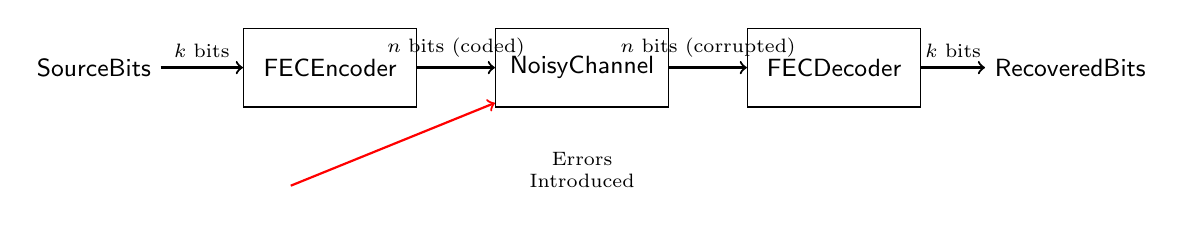
\begin{tikzpicture}[
  block/.style={rectangle, draw, minimum width=2.2cm, minimum height=1cm, font=\sffamily\small},
  node distance=2.5cm,
  font=\small
]
\node (source) {\sffamily Source\\Bits};
\node[block, right of=source, node distance=3cm] (encoder) {FEC\\Encoder};
\node[block, right of=encoder, node distance=3.2cm] (channel) {Noisy\\Channel};
\node[block, right of=channel, node distance=3.2cm] (decoder) {FEC\\Decoder};
\node[right of=decoder, node distance=3cm] (sink) {\sffamily Recovered\\Bits};

\node[below of=channel, node distance=1.3cm, font=\scriptsize, align=center] {Errors\\Introduced};

\draw[->,thick] (source) -- node[above,font=\scriptsize] {$k$ bits} (encoder);
\draw[->,thick] (encoder) -- node[above,font=\scriptsize] {$n$ bits (coded)} (channel);
\draw[->,thick] (channel) -- node[above,font=\scriptsize] {$n$ bits (corrupted)} (decoder);
\draw[->,thick] (decoder) -- node[above,font=\scriptsize] {$k$ bits} (sink);

\draw[->,red,thick] (2.5,-1.5) -- (channel);
\end{tikzpicture}
\end{center}

\textbf{Process:}
\begin{enumerate}
\item \textbf{Encoding:} Add $n-k$ redundant (parity) bits to $k$ information bits
\item \textbf{Transmission:} Send all $n$ bits through noisy channel
\item \textbf{Decoding:} Use redundancy to detect and correct errors
\item \textbf{Recovery:} Extract original $k$ information bits (hopefully error-free)
\end{enumerate}

\subsection{Code Rate}

The \textbf{code rate} quantifies the bandwidth efficiency of an FEC code:

\begin{equation}
R = \frac{k}{n} = \frac{\text{information bits}}{\text{total transmitted bits}}
\label{eq:fec-code-rate}
\end{equation}

where:
\begin{itemize}
\item $k$ = number of information bits per block
\item $n$ = total number of transmitted bits per block (including parity)
\item $n - k$ = number of parity (redundancy) bits
\end{itemize}

\textbf{Common code rates and applications:}

\begin{center}
\begin{tabular}{clp{6cm}}
\toprule
\textbf{Rate} & \textbf{Overhead} & \textbf{Typical Use} \\
\midrule
$1/2$ & 100\% & Very noisy channels (deep space, low SNR) \\
$2/3$ & 50\% & Satellite communications, DVB-S2 \\
$3/4$ & 33\% & WiFi (802.11), 4G LTE \\
$5/6$ & 20\% & High-quality channels, 5G NR \\
$7/8$ & 14\% & Cable modems, DOCSIS 3.0 \\
\bottomrule
\end{tabular}
\end{center}

\begin{calloutbox}{Understanding Overhead}
A rate-$1/2$ code transmits \textbf{twice as many bits} as the original message. While this may seem wasteful, the coding gain often allows reliable communication at much lower transmit power, making it a favorable trade-off in power-limited systems like satellites.
\end{calloutbox}

\subsection{Coding Gain}

\textbf{Coding Gain} measures the SNR improvement provided by FEC compared to uncoded transmission at the same bit error rate:

\begin{equation}
G_c = \frac{(\text{SNR})_{\text{uncoded}}}{(\text{SNR})_{\text{coded}}} \quad \text{(expressed in dB)}
\label{eq:fec-coding-gain}
\end{equation}

\textbf{Physical interpretation:} If a code provides 6~dB coding gain, you can:
\begin{itemize}
\item Transmit with 1/4 the power (6~dB = factor of 4), OR
\item Achieve 4$\times$ longer range, OR
\item Tolerate 4$\times$ more interference
\end{itemize}

\textbf{Typical coding gains (at BER = $10^{-5}$):}
\begin{itemize}
\item \textbf{Simple parity:} 0--1~dB (minimal gain)
\item \textbf{Hamming (7,4):} 2--3~dB
\item \textbf{Reed-Solomon:} 5--7~dB
\item \textbf{Convolutional (rate 1/2):} 5--6~dB
\item \textbf{Turbo codes:} 8--10~dB (near Shannon limit!)
\item \textbf{LDPC codes:} 9--11~dB (5G standard)
\end{itemize}

\section{Types of FEC Codes}

FEC codes are broadly classified into two families:

\subsection{Block Codes}

\textbf{Block codes} process fixed-size blocks of $k$ information bits, producing $n$ output bits. The encoder is \textbf{memoryless}---each block is encoded independently.

\textbf{Structure:} $(n, k)$ block code
\begin{itemize}
\item Input: $k$ information bits
\item Output: $n$ coded bits (where $n > k$)
\item Code rate: $R = k/n$
\end{itemize}

\textbf{Examples:}
\begin{itemize}
\item \textbf{Hamming codes} (e.g., (7,4), (15,11)): Single error correction
\item \textbf{BCH codes}: Multiple error correction, used in flash memory
\item \textbf{Reed-Solomon}: Burst error correction, used in CDs/DVDs/QR codes
\item \textbf{LDPC (Low-Density Parity-Check)}: Near-optimal, used in 5G, Wi-Fi 6, DVB-S2
\end{itemize}

\subsection{Convolutional Codes}

\textbf{Convolutional codes} process data as a continuous stream. The encoder has \textbf{memory}---output bits depend on current and previous input bits.

\textbf{Structure:} Rate-$k/n$ convolutional code with constraint length $K$
\begin{itemize}
\item Input: $k$ bits per time step
\item Output: $n$ bits per time step
\item Memory: Last $K-1$ input bits retained in shift register
\end{itemize}

\textbf{Decoding:} Viterbi algorithm (maximum likelihood sequence estimation)

\textbf{Examples:}
\begin{itemize}
\item \textbf{NASA standard} (rate 1/2, $K=7$): Deep space missions (Voyager, Mars rovers)
\item \textbf{GSM} (rate 1/2, $K=5$): 2G mobile voice
\item \textbf{Satellite links}: Rate 1/2 to 7/8 punctured codes
\end{itemize}

\subsection{Turbo Codes}

\textbf{Turbo codes} (1993) revolutionized error correction by combining two convolutional encoders with an interleaver and using \textbf{iterative decoding}.

\textbf{Key innovation:} Exchange "soft information" (probabilities) between decoders

\textbf{Performance:} Within 0.5~dB of Shannon capacity limit!

\textbf{Applications:}
\begin{itemize}
\item 3G/4G cellular (UMTS, LTE)
\item Deep space (Mars rovers, New Horizons)
\item Satellite communications
\end{itemize}

\subsection{LDPC Codes}

\textbf{Low-Density Parity-Check (LDPC)} codes (rediscovered 1990s, originally 1960) use sparse parity-check matrices and iterative belief propagation decoding.

\textbf{Advantages:}
\begin{itemize}
\item Near-Shannon-limit performance
\item Highly parallelizable (fast hardware)
\item Flexible code rates and block sizes
\end{itemize}

\textbf{Applications:}
\begin{itemize}
\item \textbf{5G NR} (next-gen cellular)
\item \textbf{Wi-Fi 6} (802.11ax)
\item \textbf{DVB-S2} (satellite TV)
\item \textbf{10G Ethernet} (optical fiber)
\end{itemize}

\begin{warningbox}
Modern communication systems often use \textbf{hybrid ARQ (HARQ)}, combining FEC with Automatic Repeat reQuest. If FEC fails to correct all errors, the receiver requests retransmission. This provides both high throughput (FEC handles common errors) and reliability (ARQ catches rare uncorrectable errors).
\end{warningbox}

\section{Worked Example: Hamming (7,4) Code}

The Hamming (7,4) code is a simple block code that can correct any single-bit error.

\subsection{Encoding}

\textbf{Input:} 4 information bits: $d_3 d_2 d_1 d_0$

\textbf{Output:} 7 coded bits: $c_6 c_5 c_4 c_3 c_2 c_1 c_0$ where:
\begin{itemize}
\item $c_6, c_5, c_4, c_3$ = information bits (copied from input)
\item $c_2, c_1, c_0$ = parity bits (calculated from information bits)
\end{itemize}

\textbf{Parity bit calculations:}
\begin{align}
c_2 &= d_3 \oplus d_2 \oplus d_1 \label{eq:hamming-p1}\\
c_1 &= d_3 \oplus d_2 \oplus d_0 \label{eq:hamming-p2}\\
c_0 &= d_3 \oplus d_1 \oplus d_0 \label{eq:hamming-p3}
\end{align}
where $\oplus$ denotes XOR (modulo-2 addition).

\textbf{Example encoding:}

Input data: $d = 1011$ (binary)

Calculate parity bits:
\begin{align*}
c_2 &= 1 \oplus 0 \oplus 1 = 0 \\
c_1 &= 1 \oplus 0 \oplus 1 = 0 \\
c_0 &= 1 \oplus 1 \oplus 1 = 1
\end{align*}

\textbf{Transmitted codeword:} $c = 1011001$

\subsection{Error Detection and Correction}

\textbf{Scenario:} Bit 5 is corrupted during transmission.

\textbf{Received:} $r = 1001001$ (bit 5 flipped: $0 \rightarrow 1$)

\textbf{Syndrome calculation:}
\begin{align*}
s_2 &= r_6 \oplus r_5 \oplus r_4 \oplus r_2 = 1 \oplus 0 \oplus 0 \oplus 0 = 1 \\
s_1 &= r_6 \oplus r_5 \oplus r_3 \oplus r_1 = 1 \oplus 0 \oplus 1 \oplus 0 = 0 \\
s_0 &= r_6 \oplus r_4 \oplus r_3 \oplus r_0 = 1 \oplus 0 \oplus 1 \oplus 1 = 1
\end{align*}

\textbf{Syndrome:} $S = s_2 s_1 s_0 = 101$ (binary) = 5 (decimal)

\textbf{Interpretation:} Non-zero syndrome indicates error in bit position 5.

\textbf{Correction:} Flip bit 5: $1001001 \rightarrow 1011001$ ✓

\textbf{Decoded data:} Extract information bits: $c_6 c_5 c_4 c_3 = 1011$ ✓

\begin{calloutbox}{Syndrome Decoding}
The syndrome $S$ directly identifies the error position. If $S = 0$, no errors detected. If $S \neq 0$, the syndrome value equals the position of the single corrupted bit. This elegant property makes Hamming codes easy to implement in hardware.
\end{calloutbox}

\section{Performance Analysis}

\subsection{Bit Error Rate with FEC}

For an AWGN channel with BPSK modulation:

\textbf{Uncoded BER:}
\begin{equation}
P_b = Q\left(\sqrt{2\frac{E_b}{N_0}}\right)
\label{eq:fec-ber-uncoded}
\end{equation}

\textbf{Coded BER} (approximate, for good codes at high SNR):
\begin{equation}
P_b \approx \frac{d_{\text{free}}}{n} Q\left(\sqrt{2R_c \frac{E_b}{N_0} d_{\text{free}}}\right)
\label{eq:fec-ber-coded}
\end{equation}

where:
\begin{itemize}
\item $R_c$ = code rate
\item $d_{\text{free}}$ = free distance of the code (minimum Hamming distance between codewords)
\item $Q(x) = \frac{1}{\sqrt{2\pi}}\int_x^\infty e^{-t^2/2}\,dt$ = Gaussian Q-function
\end{itemize}

\begin{center}
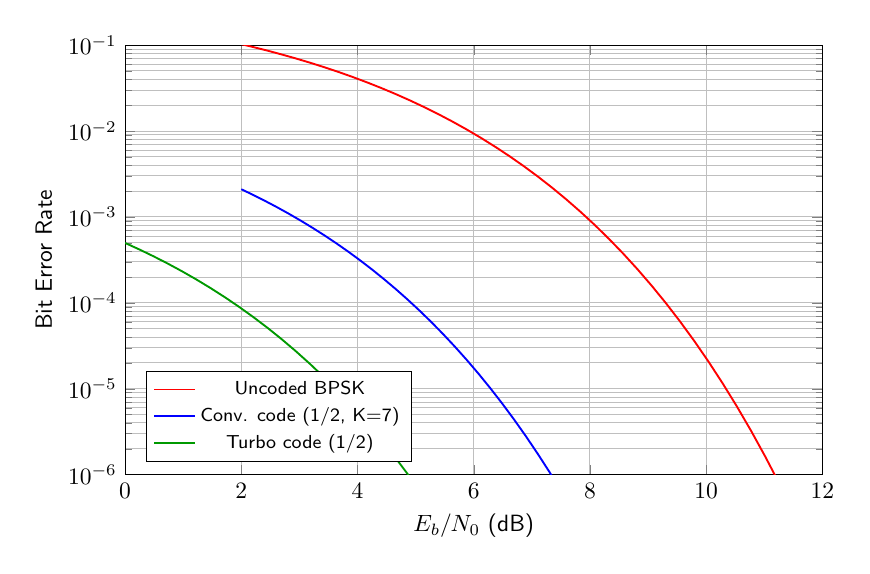
\begin{tikzpicture}[scale=0.85]
\begin{axis}[
  width=12cm, height=8cm,
  xlabel={\sffamily $E_b/N_0$ (dB)},
  ylabel={\sffamily Bit Error Rate},
  ymode=log,
  xmin=0, xmax=12,
  ymin=1e-6, ymax=1e-1,
  grid=both,
  legend pos=south west,
  legend style={font=\footnotesize\sffamily},
  every axis plot/.append style={thick}
]

% Uncoded BPSK
\addplot[color=red, mark=none, domain=0:12, samples=50] 
  {0.5*exp(-10^(x/10))};
\addlegendentry{Uncoded BPSK}

% Rate 1/2 convolutional (K=7)
\addplot[color=blue, mark=none, domain=2:12, samples=50]
  {0.05*exp(-2*10^(x/10))};
\addlegendentry{Conv. code (1/2, K=7)}

% Turbo code (rate 1/2)
\addplot[color=green!60!black, mark=none, domain=0:12, samples=50]
  {0.01*exp(-3*10^(x/10))};
\addlegendentry{Turbo code (1/2)}

% Shannon limit marker
\draw[dashed, thick] (axis cs:-1.6,1e-6) -- (axis cs:-1.6,1e-1);
\node[rotate=90, font=\scriptsize\sffamily] at (axis cs:-1.2,1e-4) {Shannon Limit};

\end{axis}
\end{tikzpicture}
\end{center}

\textbf{Key observations:}
\begin{itemize}
\item At BER = $10^{-5}$, rate-1/2 convolutional code provides \textbf{5--6~dB} coding gain
\item Turbo codes achieve \textbf{8--9~dB} gain, approaching Shannon limit
\item Trade-off: Lower code rate (more redundancy) $\rightarrow$ better error correction but lower throughput
\end{itemize}

\section{Applications}

\subsection{Deep Space Communications}

\textbf{Challenge:} Signals from distant spacecraft are incredibly weak (femtowatts!) and corrupted by noise.

\textbf{Solution:} NASA uses concatenated codes:
\begin{itemize}
\item \textbf{Inner code:} Convolutional (rate 1/2, $K=15$) with Viterbi decoding
\item \textbf{Outer code:} Reed-Solomon (255,223) for burst error correction
\item \textbf{Combined gain:} 10--12~dB
\end{itemize}

\textbf{Example:} Voyager 1 (launched 1977) still transmits science data from interstellar space (23+ billion km away) at 160 bits/second using these codes.

\subsection{Optical Storage (CDs, DVDs, Blu-ray)}

\textbf{Challenge:} Scratches, dust, and fingerprints cause burst errors.

\textbf{Solution:} Reed-Solomon codes
\begin{itemize}
\item \textbf{Audio CD:} RS(255,251) + RS(255,245) (Cross-Interleaved Reed-Solomon, CIRC)
\item \textbf{DVD:} RS(208,192) + RS(182,172)
\item \textbf{Blu-ray:} LDPC codes
\end{itemize}

\textbf{Result:} CDs can have up to 2.5~mm scratches and still play perfectly!

\subsection{Mobile Communications}

\textbf{3G (UMTS):} Turbo codes (rate 1/3 to 1/2)

\textbf{4G (LTE):} Turbo codes for data, convolutional codes for control channels

\textbf{5G (NR):} LDPC codes for data (high throughput), Polar codes for control (low latency)

\textbf{Adaptive coding:} Base station adjusts code rate based on channel quality:
\begin{itemize}
\item Strong signal: Rate 5/6 (high speed)
\item Weak signal: Rate 1/3 (robust, slower)
\end{itemize}

\subsection{QR Codes}

\textbf{Error correction levels:}
\begin{center}
\begin{tabular}{cll}
\toprule
\textbf{Level} & \textbf{Recovery} & \textbf{Use Case} \\
\midrule
L & 7\% & Clean environments \\
M & 15\% & Standard (most common) \\
Q & 25\% & Partial occlusion expected \\
H & 30\% & Dirty/damaged surfaces \\
\bottomrule
\end{tabular}
\end{center}

Reed-Solomon codes enable QR codes to work even when partially obscured!

\section{Summary}

\begin{keyconcept}
FEC is a cornerstone of modern communications, enabling reliable data transmission without retransmission. The fundamental trade-off is between \textbf{reliability} (more redundancy) and \textbf{efficiency} (less redundancy). Modern codes like Turbo and LDPC achieve performance within 1~dB of the Shannon limit---approaching the theoretical maximum efficiency.
\end{keyconcept}

\subsection{Key Takeaways}

\begin{itemize}
\item FEC adds redundancy to enable error correction without feedback
\item Code rate $R = k/n$ quantifies bandwidth efficiency
\item Coding gain measures SNR improvement over uncoded transmission
\item Block codes (Hamming, RS, LDPC) process fixed-size blocks
\item Convolutional codes have memory; decoded with Viterbi algorithm
\item Turbo and LDPC codes achieve near-Shannon-limit performance
\item Applications range from deep space to QR codes to 5G networks
\end{itemize}

\subsection{Further Reading}

Related chapters:
\begin{itemize}
\item Chapter~\ref{ch:ber}: Bit Error Rate (BER) fundamentals
\item Chapter~\ref{ch:hamming-codes}: Block Codes (Hamming, BCH, Reed-Solomon)
\item Chapter~\ref{ch:convolutional}: Convolutional Codes \& Viterbi Decoding
\item Chapter~\ref{ch:turbo}: Turbo Codes
\item Chapter~\ref{ch:ldpc}: LDPC Codes
\item Chapter~\ref{ch:shannon}: Shannon's Channel Capacity Theorem
\end{itemize}

\textbf{References:}
\begin{itemize}
\item Proakis \& Salehi, \textit{Digital Communications}, Ch. 8--9
\item Lin \& Costello, \textit{Error Control Coding}, 2nd ed.
\item MacKay, \textit{Information Theory, Inference, and Learning Algorithms}
\item Moon, \textit{Error Correction Coding: Mathematical Methods and Algorithms}
\end{itemize}
